\documentclass[a4paper]{article}

\usepackage[english]{babel}
\usepackage[utf8]{inputenc}
\usepackage{amsmath}
\usepackage{graphicx}
\usepackage[colorinlistoftodos]{todonotes}
\usepackage{float}
\usepackage{hyperref}
\usepackage{listings}
\usepackage{adjustbox}

%JUST FOR TABLE - BEGINS
\usepackage{geometry}
\usepackage{ragged2e}
\usepackage{booktabs, makecell, tabularx}
\renewcommand\theadfont{\bfseries}
\renewcommand\theadgape{}
\newcolumntype{L}{>{\RaggedRight}X}
%TABLE USER PACKAGES ENDS

\title{ENGN 8170 Group project\\ Corrosion and Gas Leaking Detection Robot\\ Project Initiation Document}

\author{U6366102, U6561524, U6622423, U6647679, U6471573}

\date{Submission date August 9, 2019}

\begin{document}
\pagenumbering{gobble}
\maketitle
\newpage
\tableofcontents
\newpage
\listoftables
\listoffigures
\newpage
\pagenumbering{arabic}
% visit https://github.com/harish-kp/Group-Project for detailed commits and updates
\section{Executive Summary}
The gas leak detection robot has more potential to grow with a variety of sensors and the nature of the environment that is to be dealt with. We propose three potential conceptual designs where, we will be analysing them theoretically and economically in the coming weeks of the semester and finalize on a single design. The concepts are differentiated by the sensor that the robot uses to sense the leak.
\begin{itemize}
    \item {Gas sensor and Pressure sensor based robot where the decision of a leak is decided by the pressure sensor.}
    \item{Infrared thermal imaging to capture the difference in temperature within the working environment.}
    \item{Internet of things} %  Pankhuri please elaborate on this point. 
\end{itemize}
%Sample image code
%begin{figure}[H]
 %  \centering
  % \includegraphics[width =8.5cm \textwidth]{}
   %\caption{Original image vs Noisy image}
    %label{fig:S1}
%\end{figure}
\section{Stakeholders}
In the following sub-sections, we will be identifying and listing all our stakeholders, priority, requirements for the pipeline inspection robot and their usage of the robot.Each of the stakeholders have their own Unique Identifiers (U.I.D). 
\subsection{List of Stakeholders}
The identified list of stakeholders are shown in the Figure \ref{fig:2.1}. The table \ref{2.1} lists the stakeholders of the project, description of the stakeholders, interest, power and strategy used to manage them.\\
\begin{figure}[htbp]
    \centerline{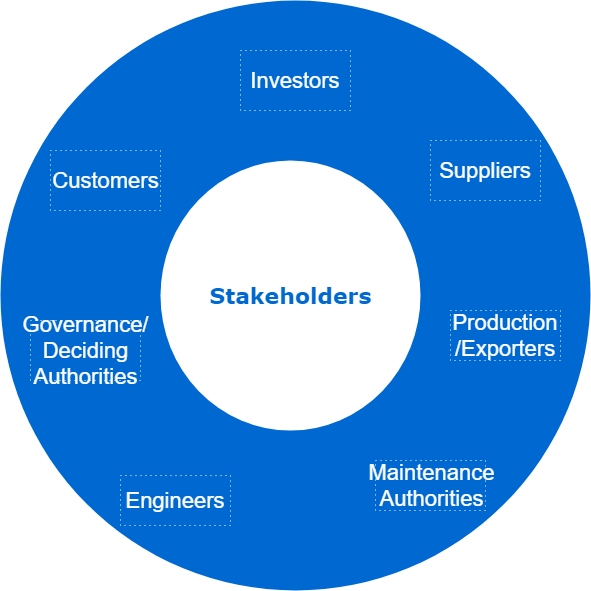
\includegraphics[width=8.5cm]{Stakeholders.png}}
    \caption{List of Stakeholders}
    \label{fig:2.1}
\end{figure}
%TABLE FOR THE STAKEHOLDERS AND THEIR PRIORITIES
\begin{table}[htb]
\caption{Details of the Stakeholders}
\label{2.1}
    \footnotesize
    \setlength\tabcolsep{3pt}
\begin{tabularx}{\linewidth}{@{} l
              >{\hsize=1.5\hsize}L
              >{\hsize=1.2\hsize}L
                            *{2}{L}*{2}{L}
                @{}}
    \toprule
\thead[b]{U.I.D}
    &   \thead{Stakeholders}
        &   \thead{Description}
            &   \thead{Interest}
                &   \thead{Power}             
                    & \thead {Strategy}\\
    \midrule
S-01  & Investors
        & Finance provider for the Project
            & High
                & High
                & Manage closely\\
    \addlinespace
S-02  & Suppliers
        & Material Supplier of the project. 
            & Low
                & Low
                    & Monitor\\
    \addlinespace
S-03   & Production/Exporters
        & Domestic and International \quad
        exporters of the products
            & Moderate
                & Low
                    & Keep informed\\
    \addlinespace
S-04   & Maintenance Authorities
        & Authorities for the safety and inspect facilities
        and resolving issues.
            & High
                & High
                    & Manage Closely\\
    \addlinespace
S-05   & Engineers
        & Team mates responsible for the designing, working and implementation of the project.
            & High
                & High
                    & Manage Closely\\
    \addlinespace
S-06   & Governance/ Deciding Authorities
        & Authorities responsible for the decision and changes in the requirements.
            & High
                & High
                    & Manage Closely\\
    \addlinespace
S-07   & Customers
        & Gas company which possess long pipelines for transmission of the oil/by-products
            & Moderate
                & High
                    & Manage Closely\\
    \bottomrule
\end{tabularx}
    \end{table}
%END OF TABLE

\subsection{Expectation Matrix}
The project expectations can be identified, defined and maintained using Expectation Matrix. This can be used to track or monitor the project. Expectation Matrix is given in the table \ref{2.2} It is characterised into four following information. \\
\\
\textbf{Expectation:} Outcome of the project and expectation of the stakeholders. \\
\textbf{Priority:} Rank of the identified expectation when compared to the other ranked expectation. Levels: High, Medium and Low. \\
\textbf{Category:} Group or Category to which the expectation suits to. For example, Engineer, Project Management, Public or Finance. \\
\textbf{Responsibility:} The department that is responsible to collect and maintain the expectation matrix with high standards. \\
\textbf{Owner:} The stakeholder who is owner of the expectation. 

%EXPECTATION MATRIX TABLE BEGINS
\begin{table}[!ht]
\caption{Expectation Matrix}
\label{2.2}
    \footnotesize
    \setlength\tabcolsep{3pt}
\begin{tabularx}{\linewidth}{@{} l
              >{\hsize=0.8\hsize}L
              >{\hsize=1.2\hsize}L
                            *{2}{L}
                @{}}
    \toprule
\thead[b]{Expectation}
    &   \thead{Priority}
        &   \thead{Category}
            &   \thead{Responsbility}
                &   \thead{Owner}            \\
    \midrule
Discussions on the meetings \\shall be documented regularly to \\track the progress and decisions
    & Medium 
        & Engineering
            & All Team members
                & S-05
                    \\
    \addlinespace
The team shall meet the \\deadlines of project on time.
    & High
        & Engineering 
            & All team members
                & S-04, S-05 
                    \\
    \addlinespace
The list of equipment required \\ for the project for purchase shall \\be provided a month in advance.
    & Medium 
        & Engineering
            & All Team members
                & S-02
                    \\
    \addlinespace
The project shall be completed  by \\12-weeks of time and within \\budget of \$300.  
    & High
        & Engineering
            & All team members
                & S-01
                    \\
    \addlinespace
System shall perform the tasks \\that are mentioned in the \\expectations of the clients or \\customers.   
    & High
        & Engineering
            & All team members
                & S-05, S-06
                   \\
    \addlinespace
Device shall be well-packed with \\handling indications and \\instructions mentioned over \\the package.   & High
        & Engineering.
            & All team members
                & S-03
                    \\
    \addlinespace
Individual peer assessment shall \\be submitted on or before the \\deadline scheduled.   
    & High
        & Engineering
            & Individual Team members
                & S-05
                    \\
    \bottomrule
\end{tabularx}
\end{table}
%EM TABLE ENDS

\section {Project Background}
 - Can write about Real life scenarios like causes and consequences and this robot will solve the problem.\bigskip \\ 
 We came across numerous concepts on the implementation of gas detection robots. During our literature review we were able to understand the existing methodologies involve detection of gas leak through programmable logic controllers  and supervisory control and data acquisition. The primary reason for not implementing robot based solutions is its uncertainty (detailed in \ref{risks}) which cannot be factored even with thorough system engineering procedures. We are trying to tackle this problem and provide feasible solution which remains profitable for the oil/ gas exporters.  
\section{Expectation}

\section{Work breakdown/Schedule}

\section{Team Organisation}
Ex: Team leader, Mechanical Engineers, System engineers, Electrical engineers, Electronic engineers.
%sample bullet
%begin{itemize}
 %  \item {D0, B, tolerance are passed into the loop}
 %  \item{An atom is selected and their inter dependency with other atoms is computed in an iteration} 
 %  \item{The atom with highest correlation returns a non zero element to X}
  % \item{Residue(r) of OMP gives information about the elements that are uncorrelated with B}
 %  \item{In main loop, Obtain the signal estimate $x_{k}$}
  % \item{Compute the estimate $\hat{b_k}$ with signal estimate $x_{k}$ }
  % \item{Update residue $r_{k+1}$ $\xleftarrow{}$ $r_k - \hat{b_k}$ }
  % \item {Move on to next iteration, until maximum iterations or tolerance values are reached}
%end{itemize}
%newpage
\section{Known Constraints}
\begin{itemize}
    \item 
\end{itemize}
\section {Resources}

\section{Risks}
\label{risks}
The potential risk of the projects are being listed below
\begin{itemize}
\subsection{Engineering risks}
    \item{Robot might breakdown inside the pipe, at a section which is inaccessible from the outside.}
    \item {During operation, robot can restrict the flow-rate of the fluid.}
    \item{Multiple leaks located very close to each other can be mistaken as a single leakage point.}
    \item{Minute fracture in pipe might not be detected due to sensor noise.}
    \item{Robot performs well under test conditions, but not might fail under actual (unprecedented) condition.}
    \item{Communication stopped due to failure of bluetooth/wifi module or signals blocked due to underground pipe.}
    \item{Gas can leak inside robot’s hull, corrupting the controller}
    \item{Electrical discharge in robot’s wiring can cause an explosion in the pipe (flammable gas).}
    \item{Unpredictable number of iterations of prototyping and testing can result in deadlines not met.}
    \item{Failure to track exact location of robot can lead to an inaccurate detection of leakage location.}
\subsection{Financial risks}
    \item{Lack of funds for fabrication of robot.}
\subsection{Administrative risks}
    \item{Availability of all team members during all stages of project development cannot be ensured.}
    \item{Delay in delivery of important components (eg. Sensors) can delay the entire project.}
    \item{Lack of appropriate guidance while facing any unidentified errors during software operation can cause delays.}
    \item{ANU maker-space lab might not be available as per our requirement, thus delaying fabrication.}

\end{itemize}
\begin{thebibliography}{9}
\bibitem{AEM}
  E. Kreyszig,
  \emph{Advanced Engineering Mathematics}.
   Tenth ed. [Online]
\bibitem{Curve}
  Gurley,
  \emph{Numerical Methods Lecture 5 Curve fitting techniques},
   2001.
\bibitem{MATLAB}
  MathWorks Inc.,
  \emph{MATLab Documentation},
   2019.
\bibitem{Lecnotes}
  Dr.Miaomiao Liu,
  \emph{Lecture Notes Semester 1},
   2019.
\bibitem{data}
Y. Xu and W. Yin. \emph{A fast patch-dictionary method for whole-image recovery.} UCLA CAM report 13-38, 2013.
\end{thebibliography}
\end{document}'